\documentclass{theozettel}

%%%%%%%%%%%%%%%%%%%%%%%%%%%%%%%%%%%%%%%%%%%%%%%%%%%%%%%%%%%%%%%%%%%%%%%%%%%%%%%%%%%%%%%%%%%%%%%%%%%%%%%%%%%%%%
% page geometry
%%%%%%%%%%%%%%%%%%%%%%%%%%%%%%%%%%%%%%%%%%%%%%%%%%%%%%%%%%%%%%%%%%%%%%%%%%%%%%%%%%%%%%%%%%%%%%%%%%%%%%%%%%%%%%
\geometry{
	left=20mm,
	right=20mm,
	top=25mm,
	bottom=20mm
}
%%%%%%%%%%%%%%%%%%%%%%%%%%%%%%%%%%%%%%%%%%%%%%%%%%%%%%%%%%%%%%%%%%%%%%%%%%%%%%%%%%%%%%%%%%%%%%%%%%%%%%%%%%%%%%

\pgfplotsset{compat=1.16}

\usepackage{dsfont}
\renewcommand{\phi}{\varphi}

\theoI{5}

\begin{document}
\punkteV{5.1}{5.2}{5.3}{5.4}{5.5}

\section*{Aufgabe 5.1} Berechnen Sie die Taylorreihen der folgenden Funktionen um den Punkt $x_0$:\\
Zur Berechnung der Taylorreihe benutzen wir folgende Formel:
\begin{align*}
f\left(x\right)&=\frac{f^{\left(0\right)}\left(x_0\right)}{0!}\left(x-x_0\right)^0+\frac{f^{\left(1\right)}\left(x_0\right)}{1!}\left(x-x_0\right)^1+\frac{f^{\left(2\right)}\left(x_0\right)}{2!}\left(x-x_0\right)^2+...+\frac{f^{\left(n\right)}\left(x_0\right)}{n!}\left(x-x_0\right)^n\\
f\left(x\right)&=\sum_{n=0}^\infty\frac{f^{\left(n\right)}\left(x_0\right)}{n!}\left(x-x_0\right)^n
\end{align*}
\subsection*{a)}$f\left(x\right)=\frac{1}{1-x}, \ x_0=0$
\begin{align*}
f\left(x\right)&=\frac{1}{1-x}\\
f'\left(x\right)&=\frac{1}{\left(1-x\right)^2}\\
f''\left(x\right)&=\frac{2}{\left(1-x\right)^3}\\
f'''\left(x\right)&=\frac{6}{\left(1-x\right)^4}\\
\text{Systematik der Ableitungen erkannt:}f^{\left(n\right)}\left(x\right)&=\frac{n!}{\left(1-x\right)^{n+1}}
\end{align*}
Einsetzen der n-ten Ableitung an der Stelle $x_0$ in die Summenformel:
\begin{align*}
f\left(x\right)&=\sum_{n=0}^\infty\frac{\frac{n!}{\left(1-x_0\right)^{n+1}}}{n!}\left(x-x_0\right)^n\\
&=\sum_{n=0}^\infty\left(1-x_0\right)^{n+1}\left(x-x_0\right)^n\\
x_0=0\Rightarrow &=\sum_{n=0}^\infty\left(1\right)^{n+1}\left(x\right)^n\\
f\left(x\right)\big|_{x_0=0}=\frac{1}{1-x}\big|_{x_0=0}&=\sum_{n=0}^\infty x^n
\end{align*}
\subsection*{b)}$f\left(x\right)=\sin x, \ x_0=\frac{\pi}{2}$
\begin{align*}
f\left(x\right)&=\sin x\\
f'\left(x\right)&=\cos x\\
f''\left(x\right)&=-\sin x\\
f'''\left(x\right) &= -\cos x\\
f''''\left(x\right) &= \sin x
\end{align*}
Da $x_0=\frac{\pi}{2}$ und $\cos\frac{\pi}{2}=0$, müssen nur die Ableitungen mit $\pm\sin x$ berücksichtigt werden, dies ist jeder zweite Ableitung, dort ergibt sich durch den Vorzeichenwechsel:
\begin{align*}
n\in\mathbb{N}_0\\
f^{\left(2n\right)}\left(x\right)&=\left(-1\right)^n\sin x
\end{align*}
Nun setzen wir $f^{\left(2n\right)}\left(x\right)$ an der Stelle $x_0$ in das Schema ein, dabei muss $n$ zu $2n$ angepasst werden:
\begin{align*}
f\left(x\right)\big|_{x_0=\frac{\pi}{2}}&=\sum_{n=0}^\infty \frac{\left(-1\right)^n\sin \frac{\pi}{2}}{\left(2n\right)!}\left(x-\frac{\pi}{2}\right)^{2n}\\
f\left(x\right)\big|_{x_0=\frac{\pi}{2}}=\sin x\big|_{x_0=\frac{\pi}{2}}&=\sum_{n=0}^\infty \frac{\left(-1\right)^n}{\left(2n\right)!}\left(x-\frac{\pi}{2}\right)^{2n}
\end{align*}
\subsection*{c)}$f\left(x\right)=\arctan x, \ x_0=0$
\begin{align*}
f^{\left(0\right)}\left(x\right)&=\arctan x\\
f^{\left(1\right)}\left(x\right) &= \frac{1}{1+x^2}\\
f^{\left(2\right)}\left(x\right)&=-\frac{2x}{\left(1+x^2\right)^2}\\
f^{\left(3\right)}\left(x\right)&=-\frac{2\left(1-3x^2\right)}{\left(x^2+1\right)^3}\\
f^{\left(4\right)}\left(x\right)&= -\frac{24x\left(x^2-1\right)}{\left(1+x^2\right)^4}\\
f^{\left(5\right)}\left(x\right)&=\frac{24\left(5x^4-10x^2+1\right)}{\left(1+x^2\right)^5}\\
f^{\left(6\right)}\left(x\right)&=-\frac{240x\left(3x^4-10x^2+3\right)}{\left(1+x^2\right)^6}\\
f^{\left(7\right)}\left(x\right)&=-\frac{720\left(1-7x^6+35x^4-21x^2\right)}{\left(1+x^2\right)^7}
\end{align*}
Nun werten wir diese Ableitungen an der Stelle $x_0=0$ aus und setzen $g^{\left(0\right)}\left(x\right)=f^{\left(1\right)}\left(x\right)$:
\begin{align*}
f^{\left(0\right)}\left(x\right)&=0\\
g^{\left(0\right)}\left(x\right)=f^{\left(1\right)}\left(x\right)&= 1\\
g^{\left(1\right)}\left(x\right)=f^{\left(2\right)}\left(x\right)&=0\\
g^{\left(2\right)}\left(x\right)=f^{\left(3\right)}\left(x\right)&=-2\\
g^{\left(3\right)}\left(x\right)=f^{\left(4\right)}\left(x\right)&= 0\\
g^{\left(4\right)}\left(x\right)=f^{\left(5\right)}\left(x\right)&=24\\
g^{\left(5\right)}\left(x\right)=f^{\left(6\right)}\left(x\right)&=0\\
g^{\left(6\right)}\left(x\right)=f^{\left(7\right)}\left(x\right)&=-720
\end{align*}
Hier lässt sich ab $g^{\left(0\right)}\left(x\right)$ ein System erkennen:\\
$n\in\mathbb{N}_0$
\begin{align*}
g^{\left(2n\right)}\left(x\right)\big|_{x_0=0}=\left(-1\right)^n\left(2n\right)!
\end{align*}
Dies lässt sich in die Formel für die Taylorreihe einsetzen:
\begin{align*}
g(x)\big|_{x_0=0}&=\frac{g^{\left(0\right)}\left(0\right)}{0!}x^0+\frac{g^{\left(2\right)}\left(0\right)}{2!}x^2+\frac{g^{\left(4\right)}\left(0\right)}{4!}x^4+...+\frac{g^{\left(2n\right)}\left(0\right)}{\left(2n\right)!}x^{2n}\\
g(x)\big|_{x_0=0}&=\sum_{n=0}^\infty\frac{g^{\left(2n\right)}\left(0\right)}{\left(2n\right)!}x^{2n}\\
&=\sum_{n=0}^\infty\frac{\left(-1\right)^n\left(2n\right)!}{\left(2n\right)!}x^{2n}\\
&=\sum_{n=0}^\infty\left(-1\right)^nx^{2n}
\end{align*}
Da $\frac{1}{1+x^2}$ die Ableitung von $\arctan x$ ist, ist das Integral der Taylorreihe von $\frac{1}{1+x^2}$ die Taylorreihe von $\arctan x$. Wir dürfen auch erst das Integral berechnen und dann summieren (vgl. Hinweis):
\begin{align*}
\arctan x\big|_{x_0=0}&=\int\text{d}x \ \sum_{n=0}^\infty\left(-1\right)^nx^{2n}\\
&=\sum_{n=0}^\infty\int\text{d}x \ \left(-1\right)^nx^{2n}\\
&=\sum_{n=0}^\infty\frac{\left(-1\right)^n}{2n+1}x^{2n+1}+c
\end{align*}
Nun müssen wir nur noch $c$ anpassen, dabei muss gelten:\\
\begin{align*}
\arctan 0= 0=\sum_{n=0}^\infty\frac{\left(-1\right)^n}{2n+1}0^{2n+1}+c\\
\Rightarrow c=0
\end{align*}
Somit ergibt sich für $\arctan x$ als Taylorreihe, entwickelt um die Stelle $x_0=0$:
\begin{align*}
\arctan x=\sum_{n=0}^\infty\frac{\left(-1\right)^n}{2n+1}x^{2n+1}
\end{align*}
\subsection*{d)}Schätzen Sie ab, wie viele Terme die Sinusreihe um $x_0=0$ Sie benötigen, um den Wert von $\sin\left(0.1\right)$ auf $10^{-5}$ genau zu erhalten. Welcher Wert ergibt sich dabei?\\\\
Die Ableitungen von $\sin x$ wurden in \textbf{b)} bereits berechnet, da dieses mal aber bei $x_0=0$ ausgewertet wird, fallen die $\pm\sin x$ Ableitungen weg und die $\pm\cos x$ Ableitungen bleiben bestehen: 
\begin{align*}
n\in\mathbb{N}_0\\
f^{\left(2n+1\right)}\left(x\right)&=\left(-1\right)^n\cos x
\end{align*}
Nun setzen wir $f^{\left(2n+1\right)}\left(x\right)$ an der Stelle $x_0$ in das Schema ein, dabei muss $n$ zu $2n+1$ angepasst werden:
\begin{align*}
f\left(x\right)&=\sum_{n=0}^\infty \frac{\left(-1\right)^n\cos x_0}{\left(2n+1\right)!}\left(x-x_0\right)^{2n+1}\\
f\left(x\right)\big|_{x_0=0}&=\sum_{n=0}^\infty \frac{\left(-1\right)^n}{\left(2n+1\right)!}\left(x\right)^{2n+1}
\end{align*}
Entwickelt man nun die Taylorreihe für die ersten Polynome ergibt dies:
\begin{align*}
f\left(x\right)\big|_{x_0=0}&=x-\frac{1}{3!}x^3+\frac{1}{5!}x^5
\end{align*}
Berechnet man hiermit den Wert von $x=0.1$ ergibt dies bereits bei $x-\frac{1}{3!}x^3$:
\begin{align*}
\sin\left(0.1\right)&\simeq 0.099833\\
0.1-\frac{1}{3!}0.1^3&=0.0998\overline{3}
\end{align*}
Dies nähert bereits $\sin\left(0.1\right)$ um $10^{-5}$ genau an. Für mich war dies doch überraschend.\\
Es muss in dieser Taylorentwicklung bis zu $x^3$ entwickelt werden.\\
Dies sind zwei Entwicklungen ($n=0, \ n=1$).



\newpage
\section*{Aufgabe 5.2}
Die Differentialgleichung des eindimensionalen harmonischen Oszillators $m\ddot{x} = F(x)$ mit $F(x) = -m\omega^{2}x$ hat die allgemeine Lösung $x(t) = A\sin(\omega t) + B\cos(\omega t)$. Für die konstante Gesamtenergie des Systems gilt:
	\[
		E = \frac{m\omega^{2}}{2}(A^{2}+B^{2}) + C.
	\]
Denn: für das Potential $V$ gilt $m\omega^{2}x = -F(x) = \dv{x} V(x)$, also $V(x) = \frac{m\omega^{2}}{2}x^{2}+C$ mit $C = \const$. Für die Gesamtenergie gilt also: (bei (1) wird die trigonometrische Identität $\sin^{2} + \cos^{2} = 1$ verwendet)
	\begin{align*}
		E &= \frac{m}{2}\ddot{x} + V(x) \\
		&= \frac{m}{2}\qty(A\omega\cos(\omega t) - B\omega\sin(\omega t))^{2} + \frac{m\omega^{2}}{2}\qty(A\sin(\omega t) + B\cos(\omega t))^{2} + C \\
		&= \frac{m\omega^{2}}{2}\big(A^{2}\cos^{2}(\omega t) - 2AB\cos(\omega t)\sin(\omega t) + B^{2}\sin^{2}(\omega t) \\ & \ \ \ \ \ \ \ \ + A^{2}\sin^{2}(\omega t) + 2AB\cos(\omega t)\sin(\omega t) + B^{2}\cos^{2}(\omega t)\big) + C\\
		&= \frac{m\omega^{2}}{2}\qty(A^{2}+B^{2})\qty(\sin^{2}(\omega t) + \cos^{2}(\omega t)) + C\\
		&\stackrel{(1)}{=} \frac{m\omega^{2}}{2}\qty(A^{2}+B^{2}) + C.
	\end{align*}
Diese ist also nicht von $t$ abhängig und somit konstant. 


\newpage
\section*{Aufgabe 5.3}
In einem Spaßbad rutscht ein Massenpunkt der Masse $m$ reibungsfrei eine spiralförmige Rutschbahn hinunter. Die Spirale habe den Radius R und vollführe drei volle Umdrehungen auf einem
Höhenunterschied $h$. Die Anfangsgeschwindigkeit des Teilchens relativ zur Rutschbahn sei Null.
Berechnen Sie die Trajektorie $\sim x(t)$ in einem geeignet gewählten Koordinatensystem. Verwenden Sie dazu den Energieerhaltungssatz.

Wir wählen den Ursprung des Koordinatensystems als den Mittelpunkt der Projektion der Rutschbahn auf den Boden. Außerdem liege de Anfangspunkt $\vec{x}(0)$ der Rutschbahn in $(R, 0, h)^{T}$. \\ Hier für $h = 5$: 
	\begin{figure}[H]
	\centering
		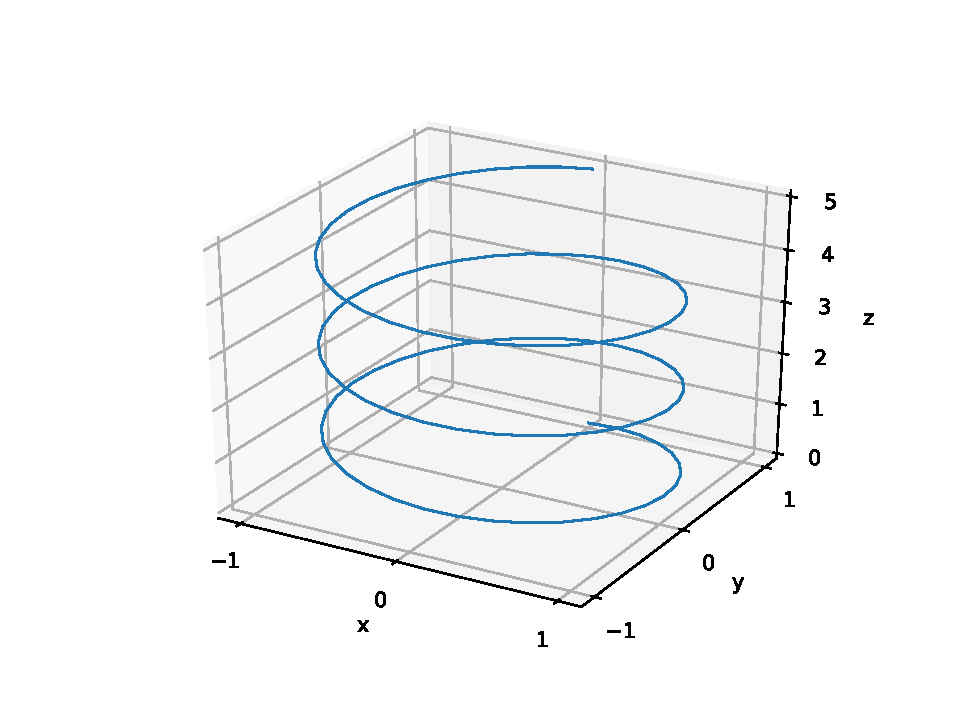
\includegraphics[scale=0.6]{plot_spiralrutsche.pdf}
	\end{figure}
	
	
Alle Punkte $\vec{x}$ der Rutschbahn lassen sich für $\phi \in [0,6\pi]$ charakterisieren durch:
	\begin{equation}
		\vec{x} = \mqty(x \\ y \\ z) = \mqty(R\cos(\phi) \\ R\sin(\phi) \\ \frac{h}{6\pi}\phi).
	\end{equation}
Sei $a=\frac{h}{6\pi}$. Für das Kraftfeld der Schwerkraft gilt $\vec{F}(x,y,z) = (0,0,mg)$ (diese wirkt lediglich in Richtung des Bodens). Für das Potential gilt $\vec{F}(\vec{x}) = -\vec{\nabla}V$. Somit erhalten wir als Potential $V(x,y,z) = mgz + C$ für $C = \const$. Da wir unser Koordinatensystem passend gewählt haben gilt $V(x,y,0) = 0$ also $C=0$. Insbesondere ist das Kraftfeld damit konservativ. Für die Gesamtenergie gilt dann also:
	\begin{align*}
		E = T + V &= \frac{m}{2}(\dot{x}^{2} + \dot{y}^{2} + \dot{z}^{2}) + mgz \\
		&= \frac{m}{2}\qty(R^{2}\sin^{2}(\phi)\dot{\phi}^{2} + R^{2}\cos^{2}(\phi)\dot{\phi}^{2} + a^{2}\dot{\phi}^{2}) + mga\phi \\
		&\stackrel{\sin^{2}+\cos^{2}=1}{=} \frac{m}{2}(R^{2}+a^{2})\dot{\phi}^{2} + mga \phi.
	\end{align*}
Energieerhaltung liefert dann:
	\begin{align*}
		& 0 = \dv{E}{t} = m(R^{2}+a^{2})\dot{\phi}\ddot{\phi} + mga\dot{\phi}\\
	\intertext{wir nehmen hier an $\dot{\phi}(t) \neq 0$ für alle $t$, da $\phi$ linear von der Bewegung in $z$-Richtung abhängt, und diese ab dem Zeitpunkt $t=0$ stets zunimmt. Dehsalb folgt:}
		\implies \ \ \ & 0 = m(R^{2}+a^{2})\ddot{\phi} + mga \\
		\implies \ \ \ & \ddot{\phi} = -\frac{ga}{(R^{2}+a^{2})} \\
		\implies \ \ \ & \dot{\phi} = -\frac{ga}{(R^{2}+a^{2})}t + C_{1} \\
		\implies \ \ \ & \phi = -\frac{ga}{2(R^{2}+a^{2})}t^{2} + C_{1}t + C_{2}.
	\end{align*}
Aus $\dot{\vec{x}}(0) = 0$ folgt $C_{1} = \dot(\phi) = \frac{6\pi}{h}\dot{z}(0) = 0$.\\ Außerdem gilt $\vec{x}(0) = (R,0,h)^{T}$, also $C_{2} = \phi(0) = \frac{6\pi}{h}z(0) = 6\pi$. Somit erhalten wir also:
	\[
		\phi(t) = -\frac{ga}{2\pi(R^{2}+a^{2})}t^{2} + 6\pi.
	\]
Setzen wir $\phi$ nun in (1) erhalten wir die Trajektorie $\vec{x} = \vec{x}(t)$. 


\newpage
\section*{Aufgabe 5.4}

Sei $\Sigma$ die vom vorgegebenen Rechteck eingeschlossene Fläche und $R$ der Rand dieser Fläche, über den beim Kurvenintegral integriert wird.

Zunächst wird das Kurvenintegral evaluiert. Da wir über das vorgegebene Rechteck integrieren, bei dessen Kanten sich jeweils nur eine Komponente ändert, gilt:

\begin{align}
\oint_R \vec{F} \cdot d \vec{s} &= \int_0^{1} F_x(s,0,0) ds + \int_0^{1} F_y(1,s,0) ds + \int_1^{0} F_x(s,1,0) ds + \int_1^{0} F_y(0,s,0) ds \\
&= \int_0^{1} F_x(s,0,0) - F_x(s,1,0) ds + \int_0^{1} F_y(1,s,0) - F_y(0,s,0) ds \\
&=  \int_0^{1} 2s^{2} - (2s^{2} - 3) ds + \int_0^{1} 0-0 ds \\
&= 3
\end{align}

Nach dem Satz von Stokes sollte dies gleich dem folgenden Flächenintegral sein:

$$
\int_\Sigma (\vec{\nabla} \times \vec{F}) \cdot d \vec{f}
$$

Da die Fläche in der $xy$-Ebene liegt, interessiert uns nur der Anteil von $(\vec{\nabla} \times \vec{F})$, der senkrecht dazu, also in $z$-Richtung ausgerichtet ist. Dieser ist:

$$
(\vec{\nabla} \times \vec{F})_z = \frac{\partial}{\partial x} 4yz - \frac{\partial}{\partial y} (2x^{2} - 3y) = 3
$$

Die Integration über die infinitesimalen Flächenelemente kann nun so aufgelößt werden, dass man zunächst über $x$ und dann über $y$ integriert:

$$
\int_\Sigma (\vec{\nabla} \times \vec{F}) \cdot d \vec{f} = \int_0^{1}  \int_0^{1} 3\ dx\ dy = 3
$$

Somit stimmt das Ergebnis überein und das Beispiel widerlegt den Satz von Stokes nicht.


\end{document}
